\documentclass[12pt,a4paper]{article}
\usepackage[left=2cm,right=2cm,top=2cm,bottom=2cm]{geometry}
\usepackage[utf8]{inputenc}
\usepackage[T2A]{fontenc}
\usepackage{amsmath}
\usepackage{amssymb}
\usepackage{graphicx}
\usepackage[russian]{babel}
\usepackage{indentfirst}
\usepackage{listings}
\usepackage{xcolor}
\usepackage{hyperref}

\hypersetup{
  colorlinks=true,
  urlcolor= blue,
  citecolor=blue,
  linkcolor= blue,
}

\title{Отчет по лабораторным работам №1-6 по дисциплине
	"Математическая статистика"}
\author{Скворцов Владимир Сергеевич (5030102/10201)}
\date{\today}

\begin{document}

	\begin{titlepage}

		\Large

		\begin{center}
			Санкт-Петербургский \\ Политехнический университет Петра Великого

			\vspace{10em}

			\textbf{Отчет по лабораторным работам №1-6} \\
			\textbf{по дисциплине}\\
			"\textbf{Математическая статистика}"

			\vspace{2em}

		\end{center}

		\vspace{6em}

		\newbox{\lbox}
		\savebox{\lbox}{\hbox{Скворцов Владимир Сергеевич}}
		\newlength{\maxl}
		\setlength{\maxl}{\wd\lbox}
		\hfill\parbox{12cm}{
			\hspace*{3cm}\hspace*{-5cm}Студент:\hfill\hbox to\maxl{Скворцов Владимир Сергеевич\hfill}\\
			\hspace*{3cm}\hspace*{-5cm}Преподаватель:\hfill\hbox to\maxl{Баженов Александр Николаевич}\\
			\\
			\hspace*{3cm}\hspace*{-5cm}Группа:\hfill\hbox to\maxl{5030102/10201}\\
		}

		\vspace{\fill}

		\begin{center}
			Санкт-Петербург \\ 2024
		\end{center}

	\end{titlepage}

	\tableofcontents

	\newpage

	\section{Постановка задачи}

	\subsection{Коэффициент корреляции}

	Сгенерировать двумерные выборки размерами 20, 60, 100 для нормального
	двумерного распределения \( N(x, y, 0, 0, 1, 1, \rho) \). Коэффициент
	корреляции \( \rho \) взять равным 0, 0.5, 0.9. Каждая выборка
	генерируется 1000 раз и для неё вычисляются: среднее значение, среднее
	значение квадрата и дисперсия коэффициентов корреля- ции Пирсона,
	Спирмена и квадрантного коэффициента корреляции. Повторить все
	вычисления для смеси нормальных распределений:

	\[
		f(x, y) = 0.9N(x, y, 0, 0, 1, 1, 0.9) + 0.1N(x, y, 0, 0, 10, 10, -0.9).
	\]

	Изобразить сгенерированные точки на плоскости и нарисовать эллипс
	равновероятности.

	\subsection{Простая линейная регрессия}

	Найти оценки коэффициентов линейной регрессии \( y_i = a + bx_i + e_i \),
	используя 20 точек на отрезке \( [-1.8; 2] \) с равномерным шагом равным
	0.2. Ошибку \( e_i \) считать нормально распределённой с параметрами
	\( (0, 1) \). В качестве эталонной зависимости взять
	\( y_i = 2 + 2x_i + e_i \). При построении оценок коэффициентов
	использовать два критерия: критерий наименьших квадратов и критерий
	наименьших модулей. Проделать то же самое для выборки, у которой в
	значения \( y_1 \) и \( y_{20} \) вносятся возмущения 10 и -10.

	\section{Теоретическое обоснование}

	\subsection{Двумерное нормальное распределение}

	Двумерная случайная величина \( (X, Y) \) называется распределённой
	нормально (или просто нормальной), если её плотность вероятности
	определена формулой

	\begin{align} \label{eq:multivariate_normal}
		N(x, y, \bar x, \bar y, \sigma_x, \sigma_y, \rho) = \frac{1}{2 \pi \sigma_x
		\sigma_y \sqrt{1 - \rho^2}} \times \exp \left \{ -\frac{1}{2(1 - \rho^2)}
		\left [ \frac{(x - \bar x)^2}{\sigma_x^2} - 2 \rho \frac{(x - \bar x)
		(y - \bar y)}{\sigma_x \sigma_y} + \frac{(y - \bar y)^2}{\sigma_y^2}
		\right ] \right \}
	\end{align}

	Компоненты \( X \), \( Y \) двумерной нормальной случайной величины также
	распределены нормально с математическими ожиданиями \( x \), \( y \) и
	средними квадратическими отклонениями \( \sigma_x \), \( \sigma_y \)
	соответственно.

	Параметр \( \rho \) называется коэффициентом корреляции.

	\subsection{Корреляционный момент (ковариация) и коэффициент корреляции}

	Корреляционный момент, иначе ковариация, двух случайных величин \( X \) и
	\( Y \):

	\begin{equation} \label{eq:covariance}
		K = \mathbf{cov}(X, Y) = \mathbf{M}[(X - \bar x)(Y - \bar y)]
	\end{equation}

	Коэффициент корреляции \( \rho \) двух случайных величин \( X \) и
	\( Y \):

	\begin{equation} \label{eq:correlation}
		\rho = \frac{K}{\sigma_x \sigma_y}
	\end{equation}

	\subsection{Выборочный коэффициент корреляции Пирсона}

	Выборочный коэффициент корреляции Пирсона:

	\begin{equation} \label{eq:pearson_corr}
		r = \frac{\frac{1}{n} \sum (x_i - \bar x)(y_i - \bar y)}{\sqrt{\frac{1}{n}
		\sum (x_i - \bar x)^2 \frac{1}{n} \sum (y_i - \bar y)^2}} =
		\frac{K}{s_X s_Y},
	\end{equation}

	где \( K \), \( s_X^2 \), \( x_Y^2 \) — выборочные ковариации и дисперсии
	случайных величин \( X \) и \( Y \).

	\subsection{Выборочный квадрантный коэффициент корреляции}

	Выборочный квадрантный коэффициент корреляции

	\begin{equation} \label{eq:quadrant_corr}
		r_Q = \frac{(n_1 + n_3) - (n_2 + n_4)}{n},
	\end{equation}

	где \( n_1 \), \( n_2 \), \( n_3 \), \( n_4 \) — количество точек с
	координатами \( (x_i, y_i) \), попавшими, соответственно, в I, II, III, IV
	квадранты декартовой системы с осями \( x' = x - \mathbf{med}x \),
	\( y' = y - \mathbf{med}y \).

	\subsection{Выборочный коэффициент ранговой корреляции Спирмена}

	Обозначим ранги, соотвествующие значениям переменной \( X \), через
	\( u \), а ранги, соотвествующие значениям переменной \( Y \), — через
	\( v \).

	Выборочный коэффициент ранговой корреляции Спирмена:

	\begin{equation}  \label{eq:spearman_corr}
		r_S = \frac{\frac{1}{n} \sum (u_i - \bar u)(v_i - \bar v)}{\sqrt{\frac{1}{n}
		\sum (u_i - \bar u)^2 \frac{1}{n} \sum (v_i - \bar v)^2}},
	\end{equation}

	где \( \bar u = \bar v = \frac{1 + 2 + \dots + n}{n} = \frac{n + 1}{2} \) —
	среднее значение рангов.

	\subsection{Эллипсы рассеивания}

	Уравнение проекции эллипса рассеивания на плоскость \( xOy \):

	\begin{equation}  \label{eq:ellipse}
		\frac{(x - \bar x)^2}{\sigma_x^2} - 2 \rho \frac{(x - \bar x)(y - \bar y)}
		{\sigma_x \sigma_y} + \frac{(y - \bar y)^2}{\sigma_y^2} = \text{const}.
	\end{equation}

	Центр эллипса \ref{eq:ellipse} находится в точке с координатами
	\( (x, y) \); оси симметрии эллипса составляют с осью \( Ox \) углы,
	определяемые уравнением

	\begin{equation}  \label{eq:ellipse}
		\tg 2 \alpha = \frac{2 \rho \sigma_x \sigma_y}{\sigma_x^2 - \sigma_y^2}.
	\end{equation}

	\subsection{Метод наименьших квадратов}

	При оценивании параметров регрессионной модели используют различные
	методы. Один из наиболее распрстранённых подходов заключается в
	следующем: вводится мера (критерий) рассогласования отклика и
	регрессионной функции, и оценки параметров регрессии определяются так,
	чтобы сделать это рассогласование наименьшим. Достаточно простые
	расчётные формулы для оценок получают при выборе критерия в виде суммы
	квадратов отклонений значений отклика от значений регрессионной функции
	(сумма квадратов остатков):

	\begin{equation} \label{eq:lsm}
		Q(\beta_0, \beta_1) = \sum \limits_{i=1}^n \varepsilon_i^2 =
		\sum \limits_{i=1}^n (y_i - \beta_0 - \beta_1 x_i)^2 \rightarrow
		\min_{\beta_0, \beta_1}.
	\end{equation}

	Задача минимизации квадратичного критерия \eqref{eq:lsm} носит название
	задачи метода наименьших квадратов (МНК), а оценки \( \beta_0 \),
	\( \beta_1 \) параметров \( \beta_0 \), \( \beta_1 \), реализующие минимум
	критерия \eqref{eq:lsm}, называют МНК-оценками.

	\subsection{Метод наименьших модулей}

	Робастность оценок коэффициентов линейной регрессии (т.е. их
	устойчивость по отношению к наличию в данных редких, но больших по
	величине выбросов) может быть обеспечена различными способами. Одним из
	них является использование метода наименьших модулей вместо метода
	наименьших квадратов:

	\begin{equation} \label{eq:lam}
		\sum \limits_{i=1}^n |y_i - \beta_0 - \beta_1 x_i| \rightarrow
		\min_{\beta_0, \beta_1}.
	\end{equation}


	\section{Описание работы}
	Лабораторные работы выполнены с использованием Python и его сторонних
	библиотек \verb!numpy!, \verb!pandas!, \verb!matplotlib!, \verb!seaborn! были
	построены гистограммы распределений и посчитаны характеристики пложения.

	Ссылка на GitHub репозиторий:
	\href{https://github.com/vladimir-skvortsov/spbstu-mathematical-statistics}
	{https://github.com/vladimir-skvortsov/spbstu-mathematical-statistics}

	\section{Результаты}

	\subsection{Коэффициент корреляции}

	\begin{table}[htbp!]
		\centering
		\begin{tabular}{ |c|c|c|c| }
			\hline
			\( n = 20 \), \( \rho = 0 \) & & & \\
			\hline
			& \( r \) \eqref{eq:pearson_corr} & \( r_S \) \eqref{eq:spearman_corr} &
			\( r_Q \) \eqref{eq:quadrant_corr} \\
			\hline
			Среднее & \( 8.051 \times 10^{-3} \) & \( 8.633 \times 10^{-3} \) &
			\( 1.216 \times 10^{-2} \) \\
			\hline
			Среднее квадратов & \( 5.501 \times 10^{-2} \) &
			\( 5.418 \times 10^{-2} \) & \( 1.033 \times 10^{-1} \) \\
			\hline
			Дисперсия & \( 5.495 \times 10^{-2} \) &
			\( 5.410 \times 10^{-2} \) & \( 1.031 \times 10^{-1} \) \\
			\hline
			\hline
			\( n = 20 \), \( \rho = 0.5 \) & & & \\
			\hline
			& \( r \) \eqref{eq:pearson_corr} & \( r_S \) \eqref{eq:spearman_corr} &
			\( r_Q \) \eqref{eq:quadrant_corr} \\
			\hline
			Среднее & \( 4.933 \times 10^{-1} \) & \( 4.674 \times 10^{-1} \) &
			\( 4.644 \times 10^{-1} \) \\
			\hline
			Среднее квадратов & \( 2.743 \times 10^{-1} \) &
			\( 2.534 \times 10^{-1} \) & \( 3.139 \times 10^{-1} \) \\
			\hline
			Дисперсия & \( 3.093 \times 10^{-2} \) &
			\( 3.496 \times 10^{-2} \) & \( 9.823 \times 10^{-2} \) \\
			\hline
			\hline
			\( n = 20 \), \( \rho = 0.9 \) & & & \\
			\hline
			& \( r \) \eqref{eq:pearson_corr} & \( r_S \) \eqref{eq:spearman_corr} &
			\( r_Q \) \eqref{eq:quadrant_corr} \\
			\hline
			Среднее & \( 8.938 \times 10^{-1} \) & \( 8.646 \times 10^{-1} \) &
			\( 9.837 \times 10^{-1} \) \\
			\hline
			Среднее квадратов & \( 8.014 \times 10^{-1} \) &
			\( 7.527 \times 10^{-1} \) & \( 1.026 \) \\
			\hline
			Дисперсия & \( 2.454 \times 10^{-3} \) &
			\( 5.209 \times 10^{-3} \) & \( 5.804 \times 10^{-2} \) \\
			\hline
			\hline
			\( n = 60 \), \( \rho = 0 \) & & & \\
			\hline
			& \( r \) \eqref{eq:pearson_corr} & \( r_S \) \eqref{eq:spearman_corr} &
			\( r_Q \) \eqref{eq:quadrant_corr} \\
			\hline
			Среднее & \( 8.143 \times 10^{-3} \) & \( 8.747 \times 10^{-3} \) &
			\( 8.485 \times 10^{-3} \) \\
			\hline
			Среднее квадратов & \( 1.709 \times 10^{-2} \) &
			\( 1.689 \times 10^{-2} \) & \( 3.111 \times 10^{-2} \) \\
			\hline
			Дисперсия & \( 1.703 \times 10^{-2} \) &
			\( 1.682 \times 10^{-2} \) & \( 3.104 \times 10^{-2} \) \\
			\hline
			\hline
			\( n = 60 \), \( \rho = 0.5 \) & & & \\
			\hline
			& \( r \) \eqref{eq:pearson_corr} & \( r_S \) \eqref{eq:spearman_corr} &
			\( r_Q \) \eqref{eq:quadrant_corr} \\
			\hline
			Среднее & \( 4.985 \times 10^{-1} \) & \( 4.757 \times 10^{-1} \) &
			\( 4.668 \times 10^{-1} \) \\
			\hline
			Среднее квадратов & \( 2.585 \times 10^{-1} \) &
			\( 2.373 \times 10^{-1} \) & \( 2.504 \times 10^{-1} \) \\
			\hline
			Дисперсия & \( 1.000 \times 10^{-2} \) &
			\( 1.094 \times 10^{-2} \) & \( 3.256 \times 10^{-2} \) \\
			\hline
			\hline
			\( n = 60 \), \( \rho = 0.9 \) & & & \\
			\hline
			& \( r \) \eqref{eq:pearson_corr} & \( r_S \) \eqref{eq:spearman_corr} &
			\( r_Q \) \eqref{eq:quadrant_corr} \\
			\hline
			Среднее & \( 8.979 \times 10^{-1} \) & \( 8.810 \times 10^{-1} \) &
			\( 9.937 \times 10^{-1} \) \\
			\hline
			Среднее квадратов & \( 8.069 \times 10^{-1} \) &
			\( 7.774 \times 10^{-1} \) & \( 1.004 \) \\
			\hline
			Дисперсия & \( 7.297 \times 10^{-4} \) &
			\( 1.202 \times 10^{-3} \) & \( 1.700 \times 10^{-2} \) \\
			\hline
			\hline
			\( n = 100 \), \( \rho = 0 \) & & & \\
			\hline
			& \( r \) \eqref{eq:pearson_corr} & \( r_S \) \eqref{eq:spearman_corr} &
			\( r_Q \) \eqref{eq:quadrant_corr} \\
			\hline
			Среднее & \( 1.396 \times 10^{-3} \) & \( 8.326 \times 10^{-5} \) &
			\( 1.584 \times 10^{-3} \) \\
			\hline
			Среднее квадратов & \( 9.856 \times 10^{-3} \) &
			\( 9.848 \times 10^{-3} \) & \( 1.972 \times 10^{-2} \) \\
			\hline
			Дисперсия & \( 9.854 \times 10^{-3} \) &
			\( 9.848 \times 10^{-3} \) & \( 1.972 \times 10^{-2} \) \\
			\hline
			\hline
			\( n = 100 \), \( \rho = 0.5 \) & & & \\
			\hline
			& \( r \) \eqref{eq:pearson_corr} & \( r_S \) \eqref{eq:spearman_corr} &
			\( r_Q \) \eqref{eq:quadrant_corr} \\
			\hline
			Среднее & \( 5.013 \times 10^{-1} \) & \( 4.812 \times 10^{-1} \) &
			\( 4.723 \times 10^{-1} \) \\
			\hline
			Среднее квадратов & \( 2.568 \times 10^{-1} \) &
			\( 2.375 \times 10^{-1} \) & \( 2.407 \times 10^{-1} \) \\
			\hline
			Дисперсия & \( 5.481 \times 10^{-3} \) &
			\( 6.013 \times 10^{-3} \) & \( 1.762 \times 10^{-2} \) \\
			\hline
			\hline
			\( n = 100 \), \( \rho = 0.9 \) & & & \\
			\hline
			& \( r \) \eqref{eq:pearson_corr} & \( r_S \) \eqref{eq:spearman_corr} &
			\( r_Q \) \eqref{eq:quadrant_corr} \\
			\hline
			Среднее & \( 8.999 \times 10^{-1} \) & \( 8.866 \times 10^{-1} \) &
			\( 1.003 \) \\
			\hline
			Среднее квадратов & \( 8.103 \times 10^{-1} \) &
			\( 7.868 \times 10^{-1} \) & \( 1.017 \) \\
			\hline
			Дисперсия & \( 4.017 \times 10^{-4} \) &
			\( 6.665 \times 10^{-4} \) & \( 1.049 \times 10^{-2} \) \\
			\hline
		\end{tabular}
		\caption{Характеристики нормального двумерного распределения}
	\end{table}

	\begin{table}[htbp!]
		\centering
		\begin{tabular}{ |c|c|c|c| }
			\hline
			\( n = 20 \) & & & \\
			\hline
			& \( r \) \eqref{eq:pearson_corr} & \( r_S \) \eqref{eq:spearman_corr} &
			\( r_Q \) \eqref{eq:quadrant_corr} \\
			\hline
			Среднее & \( -7.987 \times 10^{-2} \) & \( -7.020 \times 10^{-2} \) &
			\( -6.336 \times 10^{-2} \) \\
			\hline
			Среднее квадратов & \( 5.968 \times 10^{-2} \) &
			\( 5.944 \times 10^{-2} \) & \( 1.112 \times 10^{-1} \) \\
			\hline
			Дисперсия & \( 5.330 \times 10^{-2} \) &
			\( 5.451 \times 10^{-2} \) & \( 1.072 \times 10^{-1} \) \\
			\hline
			\hline
			\( n = 60 \) & & & \\
			\hline
			& \( r \) \eqref{eq:pearson_corr} & \( r_S \) \eqref{eq:spearman_corr} &
			\( r_Q \) \eqref{eq:quadrant_corr} \\
			\hline
			Среднее & \( 9.290 \times 10^{-2} \) & \( -8.988 \times 10^{-2} \) &
			\( -8.730 \times 10^{-2} \) \\
			\hline
			Среднее квадратов & \( 2.606 \times 10^{-2} \) &
			\( 2.553 \times 10^{-2} \) & \( 4.290 \times 10^{-2} \) \\
			\hline
			Дисперсия & \( 1.743 \times 10^{-2} \) &
			\( 1.745 \times 10^{-2} \) & \( 3.528 \times 10^{-2} \) \\
			\hline
			\hline
			\( n = 100 \) & & & \\
			\hline
			& \( r \) \eqref{eq:pearson_corr} & \( r_S \) \eqref{eq:spearman_corr} &
			\( r_Q \) \eqref{eq:quadrant_corr} \\
			\hline
			Среднее & \( -1.013 \times 10^{-1} \) & \( -9.639 \times 10^{-2} \) &
			\( -9.011 \times 10^{-2} \) \\
			\hline
			Среднее квадратов & \( 2.047 \times 10^{-2} \) &
			\( 1.984 \times 10^{-2} \) & \( 2.968 \times 10^{-2} \) \\
			\hline
			Дисперсия & \( 1.021 \times 10^{-2} \) &
			\( 1.054 \times 10^{-2} \) & \( 2.156 \times 10^{-2} \) \\
			\hline
		\end{tabular}
		\caption{Характеристики смеси нормальных распределений}
	\end{table}

	\begin{figure}[htbp!]
		\begin{center}
			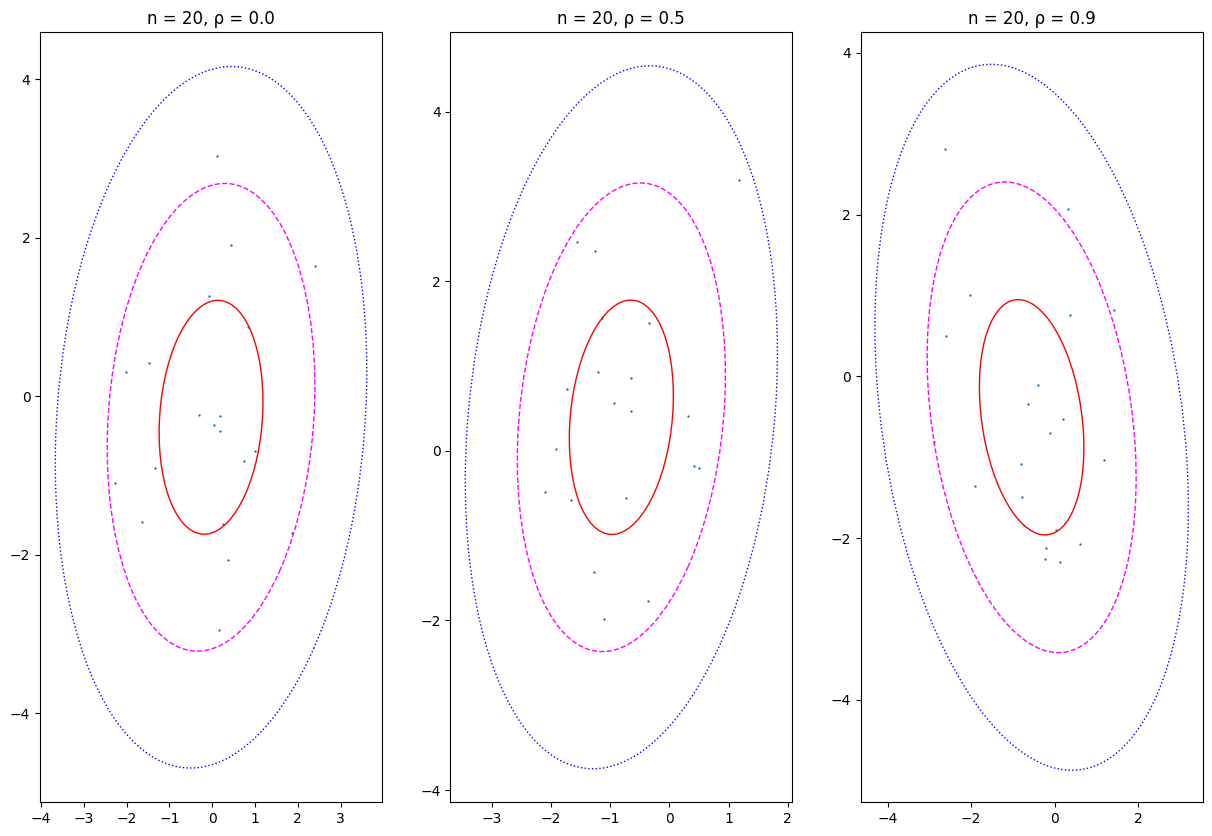
\includegraphics[width = 0.8\linewidth]{graphics/lab5_ellips_20}
			\caption{Смесь нормальных распределений и эллипсы равновероятности
			( \( n = 20 \) )}
		\end{center}
	\end{figure}

	\begin{figure}[htbp!]
		\begin{center}
			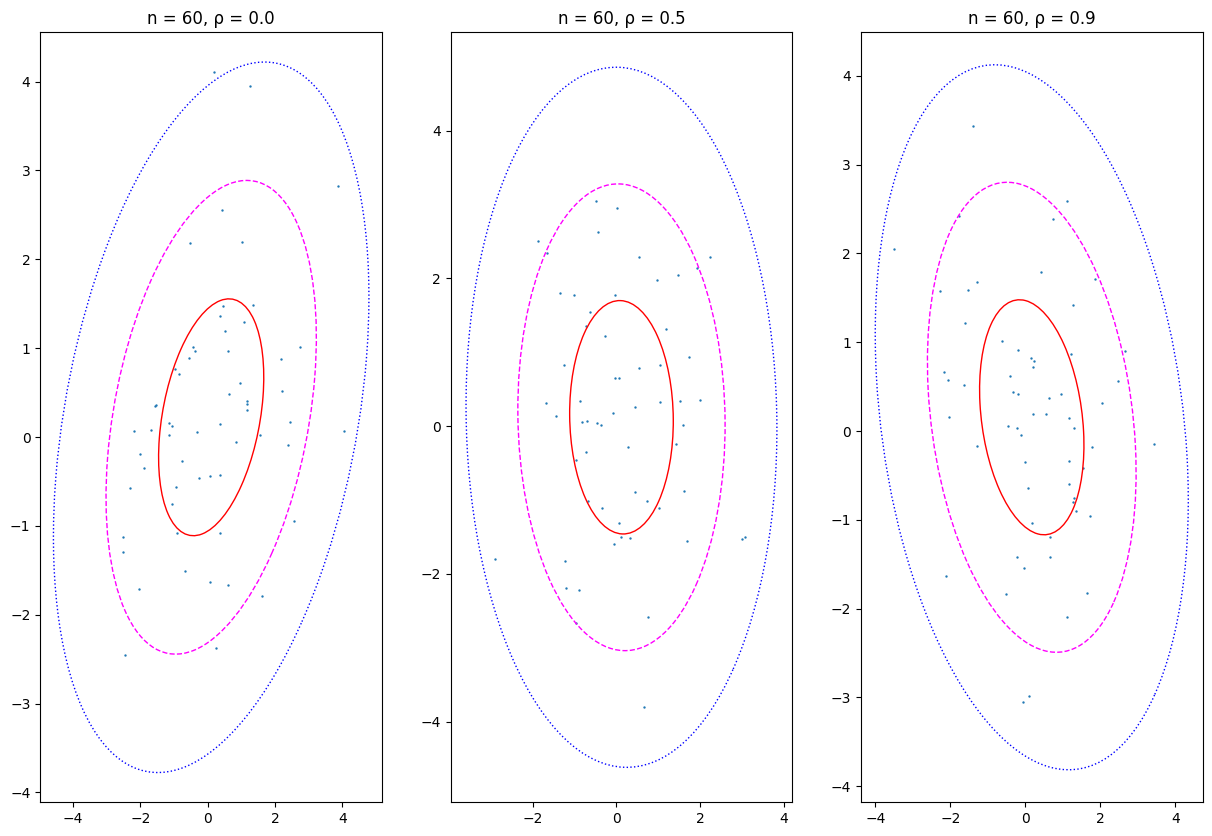
\includegraphics[width = 0.8\linewidth]{graphics/lab5_ellips_60}
			\caption{Смесь нормальных распределений и эллипсы равновероятности
			( \( n = 60 \) )}
		\end{center}
	\end{figure}

	\begin{figure}[htbp!]
		\begin{center}
			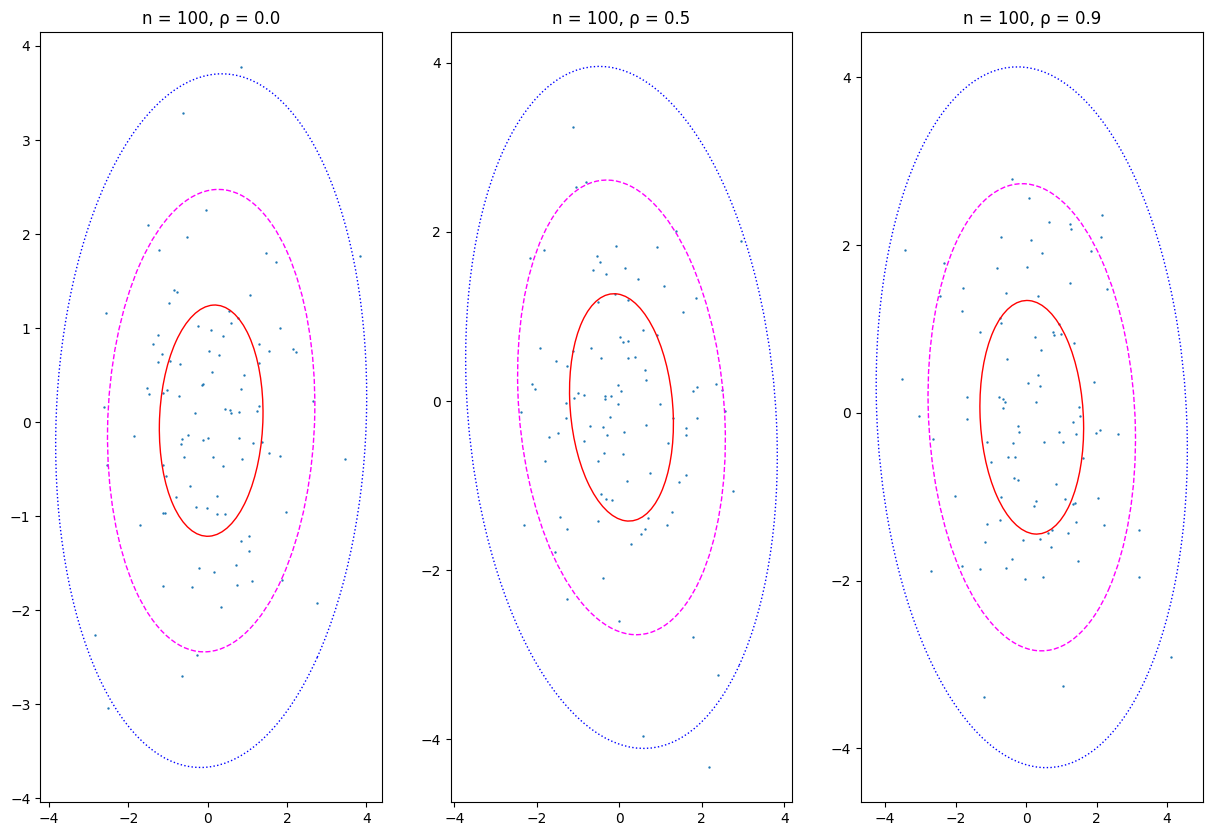
\includegraphics[width = 0.8\linewidth]{graphics/lab5_ellips_100}
			\caption{Смесь нормальных распределений и эллипсы равновероятности
			( \( n = 100 \) )}
		\end{center}
	\end{figure}

	\clearpage

	\subsection{Простая линейная регрессия}

	\begin{figure}[htbp!]
		\begin{center}
			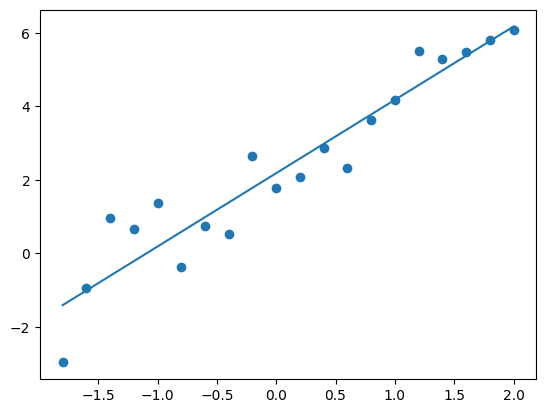
\includegraphics[width = 1\linewidth]{graphics/lab6_sq.png}
			\caption{Метод наименьших квадратов \( ( 1.861, 2.061) \)}
		\end{center}
	\end{figure}

	\begin{figure}[htbp!]
		\begin{center}
			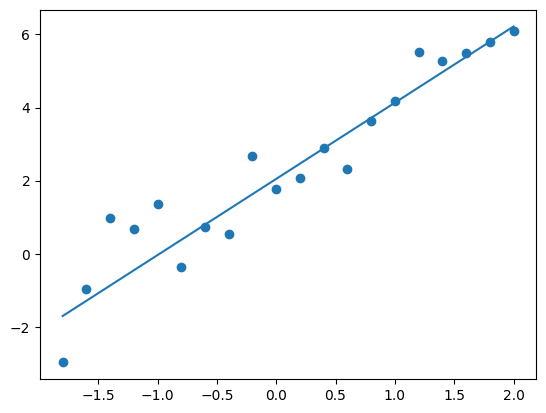
\includegraphics[width = 1\linewidth]{graphics/lab6_abs.png}
			\caption{Метод наименьших модулей \( (1.7691, 2.162) \)}
		\end{center}
	\end{figure}

	\begin{figure}[htbp!]
		\begin{center}
			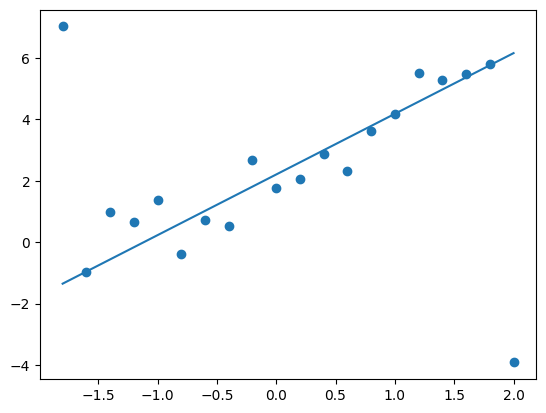
\includegraphics[width = 1\linewidth]{graphics/lab6_abs_mod.png}
			\caption{Метод наименьших квадратов с возмущениями
				\( (1.668, 1.990) \)}
		\end{center}
	\end{figure}

	\begin{figure}[htbp!]
		\begin{center}
			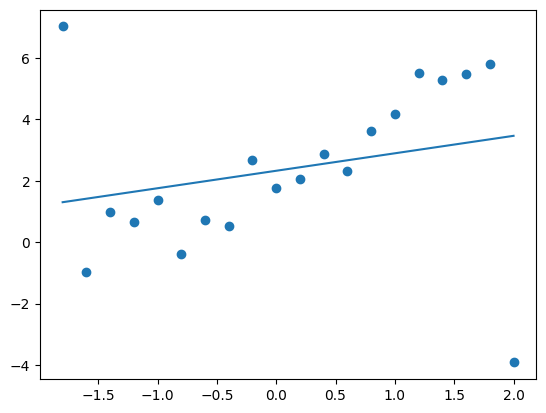
\includegraphics[width = 1\linewidth]{graphics/lab6_sq_mod.png}
			\caption{Метод наименьших модулей с возмущениями \( (2.004, 0.632) \)}
		\end{center}
	\end{figure}

	\clearpage

	\begin{table}[htbp]
		\centering
		\begin{tabular}{ |c|c|c|c|c|c|c| }
			\hline
			& \( a \)  & \( a' \) & \( b \) & \( b' \) & \( \Delta a \) & \( \Delta b \) \\
			\hline
			МНК & 2.0388 & 2.3383 & 2.1955 & 0.6102 & 1.3383 & 0.7221 \\ \hline
			МНМ & 2.3634 & 1.9944  & 1.9945 & 2.3634 & 0.1561 & 0.1849 \\ \hline
		\end{tabular}
		\caption{Таблица коэффициентов}
	\end{table}

	Здесь:

	\begin{itemize}
		\item \( y = ax + b \) — уравнение линейной регресси для методов МНК и
			МНМ без выбросов
		\item \( y = a'x + b' \) — уравнение линейной регресси для методов МНК и
			МНМ с выбросами
		\item \( \Delta a = \frac{|a - a'|}{a} \)
		\item \( \Delta b = \frac{|b - b'|}{b} \)
	\end{itemize}

	\clearpage

	\section{Выводы}

	На основе полученных характеристик (включая среднее значение, среднее
	значение квадрата и дисперсию) для различных коэффициентов корреляции и
	размеров выборки, можно сделать следующие наблюдения:

	\begin{enumerate}
		\item При увеличении размера выборки повышается точность оценок, что
		видно по уменьшению дисперсий коэффициентов корреляции. Это
		соответствует принципам центральной предельной теоремы и закона
		больших чисел.
		\item При увеличении коэффициента корреляции \( \rho \), средние
		значения коэффициентов Пирсона, Спирмена и квадратичного коэффициента
		корреляции тоже увеличиваются. Это указывает на прямую связь между
		\( \rho \) и другими коэффициентами корреляции.
	\end{enumerate}

	Из результатов оценок коэффициентов линейной регрессии при использовании
	двух критериев (критерий наименьших квадратов и критерий наименьших
	модулей) можно сделать следующие выводы:

	\begin{enumerate}
		\item Метод наименьших квадратов показал себя эффективно в случае,
		когда нет значительных выбросов в данных, в то время как метод
		наименьших модулей проявил себя лучше в присутствии значительных
		возмущений.
		\item Важно выбирать метод, исходя из особенностей данных. Если в
		данных присутствуют выбросы, метод наименьших модулей будет
		предпочтительнее из-за его устойчивости к выбросам.
	\end{enumerate}

	\section{Постановка задачи}

	\subsection{Проверка гипотезы о законе распреде- ления генеральной
		совокупности. Метод хи-квадрат}

	Создать распределения согласно нормальному, распределению Стьюдента и
	равномерному распределению с мощностями выборки \( n=20, 100 \).

	Провести исследование по методу \( \chi^2 \).

	\subsection{Проверка гипотезы о равенстве дисперсий двух нормальных
		генеральных совокупностей}

		Мощность нормального распределения \( N = 100 \).

		\begin{enumerate}
			\item Выбрать две выборки мощностью 20 и 40
			\item Выбрать две выборки мощностью 20 и 100
		\end{enumerate}

		Провести исследование по методу теста Фишера для случаев 1 и 2.

		\section{Теоретическое обоснование}

		\subsection{Проверка гипотезы о законе распреде- ления генеральной
			совокупности. Метод хи-квадрат}

		\subsection{Проверка гипотезы о равенстве дисперсий двух нормальных
			генеральных совокупностей}

		\subsubsection{Правило проверки гипотезы о законе распре- деления по
			методу \( \chi^2 \)}

		\begin{enumerate}
			\item Выбираем уровень значимости \( \alpha \),
			\item По таблице находим квантиль \( \chi_{1-\alpha}^2 (k - 1) \)
				распределения хи-квадрат с \( k - 1 \) степенями свободы порядка
				\( 1 - \alpha \),
			\item С помощью гипотетической функции распределения \( F(x) \)
				вычисляем вероятности
				\( p_i = P(X \in \Delta_i), \ i \in \overline{1,k} \),
			\item Находим частоты \( n_i \) попадания элементов выборки в
				подмножества \( \Delta_i, \ i \in \overline{1,k} \).
		\end{enumerate}

		\subsubsection{Тест Фишера}

		Несмещенные оценки дисперсий:

		\begin{equation} \label{eq:unbiased_estimations_of_dispersion}
			s_X^2 = \frac{1}{m - 1} \sum_{i=1}^m (x_i - \bar x)^2; \
			s_Y^2 = \frac{1}{n - 1} \sum_{i=1}^m (y_i - \bar y)^2;
		\end{equation}

		Статистика критерия Фишера:

		\begin{equation} \label{eq:fisher}
			F = s_X^2 / s_Y^2
		\end{equation}

		\begin{enumerate}
			\item Вычисляем несмещенные оценки дисперсий
				\eqref{eq:unbiased_estimations_of_dispersion},
			\item Выбираем статистику критерия \eqref{eq:fisher},
			\item Выбираем уровень значимости \( \alpha \),
			\item По таблице квантиль \( F_{1 - \frac{\alpha}{2}} (k_1, k2) \)
				распределения Фишера.
			\item Вычисляем выборочное значение \( F_V \) статистики критерия.
			\item Сравниваем \( F_B \) и \( F_{1 - \frac{\alpha}{2}} (k_1, k2) \).
				Если \( F_B < F_{1 - \frac{\alpha}{2}} (k_1, k2) \), то гипотеза
				\( H_0 \) на выбранном уровне значимости \( \alpha \) принимается.
				В противном случае — отвергается.
		\end{enumerate}

\end{document}
